\documentclass[11pt,a4paper,oneside]{scrartcl}

\newcommand{\mchname}{Mat\'{u}\v{s} Chochl\'{i}k}
\newcommand{\mchmail}{chochlik@gmail.com}
\newcommand{\docname}{Static reflection (rev. 2)}
\newcommand{\docnum}{N4111}
\newcommand{\docdate}{2014-07-02}

\usepackage[utf8]{inputenc}
\usepackage{url}
\usepackage[colorlinks=true]{hyperref}
\usepackage{parskip}

\usepackage{listings}
\usepackage{minted}
\lstset{basicstyle=\footnotesize\ttfamily,breaklines=true}

\usepackage{fancyhdr}
\setlength{\headheight}{14pt}
\pagestyle{fancyplain}
\lhead{\fancyplain{}{\docnum - \docname}}
\rhead{}
\rfoot{\fancyplain{}{\thepage}}
\cfoot{}

\usepackage[pdftex]{graphicx}
\DeclareGraphicsExtensions{.pdf,.png,.jpg,.mps,.eps}
\graphicspath{{images/}}

\usepackage{tikz}
\usetikzlibrary{arrows,positioning}
\tikzstyle{concept}=[
	rectangle,	
	very thick,
	draw=red!80!black!80,
	top color=white,
	bottom color=red!20,
	node distance=0.5em and 1.5em
]
\tikzstyle{inheritance}=[
	->,
	shorten >=1pt,
	>=open triangle 90,
	very thick
]
   

\setcounter{tocdepth}{3} 

\title{\docname}

\author{\mchname (\mchmail)}

\newcommand{\concept}[1]{\hyperref[concept-#1]{\em{#1}}}
\newcommand{\meta}[1]{\concept{Meta#1}}

\begin{document}

\begin{tabular}{r l}
Document number: & \docnum\\
Date: & \docdate\\
Project: & Programming Language C++, SG7, Reflection\\
Reply-to: & \mchname (\href{mailto:\mchmail}{\mchmail})\\
\end{tabular}

\begin{center}
\vskip 2em
{\Huge \docname}
\vskip 1em
{\emph \mchname}
\vskip 2em
\end{center}

\paragraph{Abstract}

In N3996 \cite{n3996} we presented some ideas on the design and possible
implementation of a compile-time reflection facility for standard C++.
N3996 also contained extensive discussion about usefulness of reflection,
description of several use-cases and motivational examples from the Mirror
reflection utilities \cite{mirror-doc-cpp11}.
The actual proposal was however found to be confusing in some points.
This paper tries to make the proposal more concise and detailed.

\tableofcontents

%\section{Introduction}

Reflection and reflective programming can be used
for a wide range of tasks such as implementation of serialization-like operations,
remote procedure calls, scripting, automated GUI-generation,
implementation of several software design patterns, etc.
C++ as one of the most prevalent programming languages 
lacks a standardized reflection facility.

In this paper we propose the addition of native support for
compile-time reflection to C++ and a library built
on top of the metadata provided by the compiler.

The basic static metadata provided by compile-time reflection
should be as complete as possible to be applicable in a wide
range of scenarios and allow to implement custom higher-level
static and dynamic reflection libraries and reflection-based
utilities.

The term \emph{reflection} refers to the ability of a computer program
to observe and possibly alter its own structure and/or its behavior.
This includes building new or altering the existing data structures,
doing changes to algorithms or changing the way the program code
is interpreted. Reflective programming is a particular kind
of \emph{metaprogramming}.

The advantage of using reflection is in the fact that everything
is implemented in a single programming language, and the human-written
code can be closely tied with the customizable reflection-based
code which is automatically generated by compiler metaprograms,
based on the metadata provided by reflection.

The solution proposed in this paper is based on the
\href{http://kifri.fri.uniza.sk/~chochlik/mirror-lib/html/}{\em Mirror}
reflection utilities~\cite{mirror-doc-cpp11} and on several years
of user experience with reflection-based metaprogramming.

\section{Metaobject concepts}

We propose that the basic metadata describing a program written
in C++ should be made available through a set of {\em anonymous} types
and related functions and templates
defined by the compiler. These types should describe various program
constructs like, namespaces, types, typedefs, classes, their member variables
(member data), member functions, inheritance, templates, template parameters,
enumerated values, etc.

The compiler should generate metadata for the program constructs defined
in the currently processed translation unit. Indexed sets (ranges) of metaobjects,
like scope members, parameters of a function, etc. should be listed
in the order of appearance in the processed source code.

Since we want the metadata to be available at compile-time,
different base-level constructs should be reflected by
{\em "statically" different} metaobjects and thus by {\em different} types.
For example a metaobject reflecting the global scope namespace should
be a different {\em type} than a metaobject reflecting the \verb@std@
namespace, a metaobject reflecting the \verb@int@ type should
have a different type then a metaobject reflecting the \verb@double@
type, a metaobject reflecting \verb@::foo(int)@ function should
have a different type than a metaobject reflecting \verb@::foo(double)@,
function, etc.

In a manner of speaking these special types (metaobjects) should become
"instances" of the meta-level concepts (static interfaces which
should not exist as concrete types, but rather only at the
"specification-level" similar for example to the iterator concepts).
This section describes a set of metaobject concepts,
their interfaces, tag types for metaobject classification and
functions (or operators) providing access to the metaobjects.

This section conceptualy describes the requirements that various metaobjects
need to satisfy in order to be considered models of the individual
concepts.

Unless stated otherwise all additions proposed and described below should
go into the \verb@std@ namespace. Alternatively, if any of the definitions
proposed here clash with existing members (or new members proposed elsewhere)
of the \verb@std@ namespace then they can be nested in a namespace like
\verb@std::meta@ or \verb@std::mirror@.

Also note, that in the sections below, the exaples use names for concrete
metaobjects with names like \verb@__meta_std_string@. This convention
is {\em NOT} part of this proposal. The actual naming of the metaobjects
should be left to the compiler implementations and for all purposes
from the users point of view the metaobjects should be anonymous types.

\subsection{Categorization and Traits}

In order to provide means for distinguishing between regular types
and metaobjects generated by the compiler,
the \verb@is_metaobject@ trait should be added
and should "return" \verb@true_type@ for metaobjects (types generated
by the compiler providing metadata) and \verb@false_type@
for non-metaobjects (native or user defined types):

\begin{lstlisting}
template <typename T>
struct is_metaobject
 : false_type
{ };
\end{lstlisting}

\subsubsection{Metaobject category tags}
\label{metaobject-category-tags}

To distiguish between various metaobject kinds (satisfying different concepts
as described below) a set of tag \verb@struct@s (indicating the kind of the metaobject)
should be added:

\begin{lstlisting}
struct specifier_tag
{
	typedef specifier_tag type;
};

struct namespace_tag
{
	typedef namespace_tag type;
};

struct global_scope_tag
{
	typedef global_scope_tag type;
};

struct type_tag
{
	typedef type_tag type;
};

struct typedef_tag
{
	typedef typedef_tag type;
}; 

struct class_tag
{
	typedef class_tag type;
};

struct function_tag
{
	typedef function_tag type;
};

struct constructor_tag
{
	typedef constructor_tag type;
};

struct operator_tag
{
	typedef operator_tag type;
};

struct overloaded_function_tag
{
	typedef overloaded_function_tag type;
};

struct enum_tag
{
	typedef enum_tag type;
};

struct enum_class_tag
{
	typedef enum_class_tag type;
};

struct inheritance_tag
{
	typedef inheritance_tag type;
};

struct constant_tag
{
	typedef constant_tag type;
};

struct variable_tag
{
	typedef variable_tag type;
};

struct parameter_tag
{
	typedef parameter_tag type;
};
\end{lstlisting}

These tags are referred-to as \verb@MetaobjectCategory@ below:

\subsubsection{Specifier category tags}
\label{specifier-category-tags}

Similar to the \hyperref[metaobject-category-tags]{metaobject tag} types,
a set of tag types for individual C++ specifier keywords should be defined:

\begin{lstlisting}
// indicates no specifier
struct none_tag
{
	typedef none_tag type;
};

struct extern_tag
{
	typedef extern_tag type;
};

struct static_tag
{
	typedef static_tag type;
};

struct mutable_tag
{
	typedef mutable_tag type;
};

struct register_tag
{
	typedef register_tag type;
};

struct thread_local_tag
{
	typedef thread_local_tag type;
};

struct const_tag
{
	typedef const_tag type;
};

struct virtual_tag
{
	typedef virtual_tag type;
};

struct private_tag
{
	typedef private_tag type;
};

struct protected_tag
{
	typedef protected_tag type;
};

struct public_tag
{
	typedef public_tag type;
};

struct class_tag
{
	typedef class_tag type;
};

struct struct_tag
{
	typedef struct_tag type;
};

struct union_tag
{
	typedef union_tag type;
};

struct enum_tag
{
	typedef enum_tag type;
};

struct enum_class_tag
{
	typedef enum_class_tag type;
};

struct constexpr_tag
{
	typedef constexpr_tag type;
};

\end{lstlisting}

These tags are collectively referred-to as \verb@SpecifierCategory@ below.

\subsection{StringConstant}
\label{concept-StringConstant}

A \concept{StringConstant} is a class conforming to the following:

\begin{lstlisting}
struct StringConstant
{
	typedef StringConstant type;

	// null terminated char array
        static constexpr const char value[Length+1] = {..., '\0'};

	// implicit conversion to null terminated c-string
        constexpr operator const char* (void) const
        {
                return value;
        }
};

constexpr const char StringConstant::value[Length+1];
\end{lstlisting}

Concrete models of \concept{StringConstant} are used to return compile-time string values.
For example the \verb@_str_void@ type defined below, conforms to the \concept{StringConstant}
concept:

\begin{lstlisting}
template <char ... C>
struct string_constant
{
	typedef string_constant type;

	static constexpr const char value[sizeof...(C)+1] = {C...,'\0'};

	constexpr operator const char* (void) const
	{
		return value;
	}
};

template <char ... C>
constexpr const char string_constant::value[sizeof...(C)+1];

//...

typedef string_constant<'v','o','i','d'> _str_void;

cout << _str_void::value << std::endl;
cout << _str_void() << std::endl;
static_assert(sizeof(_str_void::value) == 4+1, "");
\end{lstlisting}

The strings stored in the \verb@value@ array should be UTF-8 encoded.

Also note, that the \verb@string_constant@ class as defined above is just one of the
possible implementations of \concept{StringConstant}, we do not however imply
that it must be implemented this way.

\subsection{Metaobject Sequence}
\label{concept-MetaobjectSequence}

As the name implies \concept{MetaobjectSequence}s are used to store seqences
of metaobjects.
A model of \concept{MetaobjectSequence} is a class conforming to the following:

It is a nullary metafunction returning itself:

\begin{lstlisting}
template <typename Metaobject>
struct MetaobjectSequence
{
	typedef MetaobjectSequence type;
};
\end{lstlisting}

Note that the above is only a psedo-code and
the template parameter \verb@Metaobject@ indicates here the minimal
metaobject concept which all elements in the sequence must satisfy.
For example a \verb@MetaobjectSequence<MetaConstructor>@ denotes a sequence
of metaobjects that all satisfy the \meta{Constructor} concept, etc.

\subsubsection{\texttt{size}}

A template class \verb@size@ is defined as follows:

\begin{lstlisting}
template <typename T>
struct size;

template <>
struct size<MetaobjectSequence<Metaobject>>
 : integral_type<size_t, N>
{ };
\end{lstlisting}

Where \verb@N@ is the number of elements in the sequence.

\subsubsection{\texttt{at}}

A template class \verb@at@, providing random access to metaobjects in a sequence
is defined (for values of \verb@I@ between \verb@0@ and \verb@N-1@ where \verb@N@
is the number of elements returned by \verb@size@) as follows:

\begin{lstlisting}
template <typename T, size_t I>
struct at;

template <size_t I>
struct at<MetaobjectSequence<Metaobject>, I>
 : Metaobject
{ };
\end{lstlisting}


\subsection{Metaobject}
\label{concept-Metaobject}

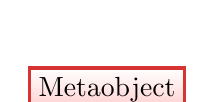
\begin{tikzpicture}
\node[concept] (Metaobject) {Metaobject};
\end{tikzpicture}

A \meta{object} is a stateless anonymous type generated by the compiler which
provides metadata reflecting a specific program feature. Each metaobject
should satisfy the following:

Every metaobject should be a nullary metafunction returning itself:

\begin{minted}{cpp}
struct Metaobject
{
	typedef Metaobject type;
};
\end{minted}

The \verb@is_metaobject@ template should return \verb@true_type@.

\begin{minted}{cpp}
template <>
struct is_metaobject<Metaobject>
 : true_type
{ };
\end{minted}

\subsubsection{\texttt{metaobject\_category}}

A template class \verb@metaobject_category@ should be defined in the \verb@std@ namespace
(even if everything else is defined inside of a nested namespace like \verb@std::meta@)
and should inherit from
one of the \hyperref[metaobject-category-tags]{metaobject category tags}, depending on
the actual kind of the metaobject.

\begin{minted}{cpp}
template <typename T>
struct metaobject_category;

template <>
struct metaobject_category<Metaobject>
 : MetaobjectCategory
{ };
\end{minted}

For example if the \verb@__meta_std@ metaobject reflects the \verb@std@ namespace,
then the specialization of \verb@metaobject_category@ should be:

\begin{minted}{cpp}
template <>
struct metaobject_category<__meta_std>
 : namespace_tag
{ };
\end{minted}

\subsubsection{Traits}

The following template classes indicating various properties of a \meta{object}
should be defined and should by default inherit from \verb@false_type@ unless stated
otherwise below:

\verb@has_name@ -- indicates that a \meta{object} is a \meta{Named}:
\begin{minted}{cpp}
template <typename T>
struct has_name
 : false_type
{ };
\end{minted}

\verb@has_scope@ -- indicates that a \meta{object} is a \meta{Scoped}:
\begin{minted}{cpp}
template <typename T>
struct has_scope
 : false_type
{ };
\end{minted}

\verb@is_scope@ -- indicates that a \meta{object} is a \meta{Scope}:
\begin{minted}{cpp}
template <typename T>
struct is_scope
 : false_type
{ };
\end{minted}

\verb@is_class_member@ -- indicates that a \meta{object} is a \meta{ClassMember}:
\begin{minted}{cpp}
template <typename T>
struct is_class_member
 : false_type
{ };
\end{minted}

\verb@has_template@ -- indicates that a \meta{object} is a \meta{Instantiation}:
\begin{minted}{cpp}
template <typename T>
struct has_template
 : false_type
{ };
\end{minted}

\verb@is_template@ -- indicates that a \meta{object} is a \meta{Template}
or \meta{TemplateParameter}:
\begin{minted}{cpp}
template <typename T>
struct is_template
 : false_type
{ };
\end{minted}


\subsection{MetaSpecifier}
\label{concept-MetaSpecifier}

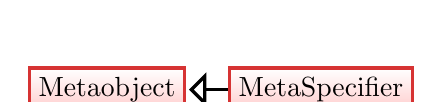
\begin{tikzpicture}
\node[concept] (Metaobject) {Metaobject};
\node[concept] (MetaSpecifier) [right=of Metaobject] {MetaSpecifier}
	edge[inheritance] (Metaobject);
\end{tikzpicture}

\meta{Specifier} is a \meta{object} reflecting a C++ specifier. In addition to the requirements
inherited from \meta{object}, types conforming to this concept must satisfy the following:

The \verb@metaobject_category@ template should return \verb@specifier_tag@ for all \meta{Specifiers}.

\begin{lstlisting}
template <>
struct metaobject_category<MetaSpecifier>
 : specifier_tag
{ };
\end{lstlisting}

\subsubsection{\texttt{specifier\_category}}

A template struct \verb@specifier_category@ should be defined and should inherit from one of the
\hyperref[specifier-category-tags]{specifier category tags}, depending on
the actual reflected specifier.

\begin{lstlisting}
template <typename T>
struct specifier_category;

template <>
struct specifier_category<MetaSpecifier>
 : SpecifierCategory
{ };
\end{lstlisting}

For example if the \verb@__meta_static@ metaobject reflects the \verb@static@
C++ specifier, then the specialization of \verb@specifier_category@
should be:

\begin{lstlisting}
template <>
struct specifier_category<__meta_static>
 : static_tag
{ };
\end{lstlisting}


\subsubsection{\texttt{keyword}}

A template struct \verb@keyword@ should be defined and should return
the keyword matching the reflected specifier as a
\concept{StringConstant}.

\begin{lstlisting}
template <typename T>
struct keyword;

template <>
struct keyword_category<MetaSpecifier>
 : StringConstant
{ };
\end{lstlisting}

For example if the \verb@__meta_thread_local@ metaobject reflects the \verb@thread local@
specifier, then the matching specialization of \verb@keyword@ could be following:

\begin{lstlisting}
template <>
struct keyword<__meta_thread_local>
 : string_constant<'t','h','r','e','a','d',' ','l','o','c','a','l'>
{ };
\end{lstlisting}

The \verb@string_constant<'t','h','r','e','a','d',' ','l','o','c','a','l'>@
class should be a model of \concept{StringConstant} as described above.


\subsection{MetaNamed}
\label{concept-MetaNamed}

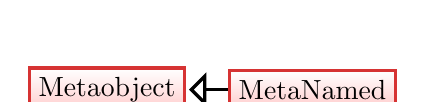
\begin{tikzpicture}
\node[concept] (Metaobject) {Metaobject};
\node[concept] (MetaNamed) [right=of Metaobject] {MetaNamed}
	edge[inheritance] (Metaobject);
\end{tikzpicture}

\meta{Named} is a \meta{object} reflecting program constructs, which have a name
(are identified by an identifier) like namespaces, types, functions, variables, parameters, etc.

In addition to the requirements inherited from \meta{object}, the following requirements must
be satisfied:

The \verb@has_name@ template class specialization for a \meta{Named} should
inherit from \verb@true_type@:

\begin{minted}{cpp}
template <>
struct has_name<MetaNamed>
 : true_type
{ };
\end{minted}

\subsubsection{\texttt{base\_name}}

A template class \verb@base_name@ should be defined an should return the base name
of the reflected construct, without the nested name specifier nor any qualifications
or other decorations, as a
\concept{StringConstant}:

\begin{minted}{cpp}
template <typename T>
struct base_name;

template <>
struct base_name<MetaNamed>
 : StringConstant
{ };
\end{minted}

For example, if \verb@__meta_std_size_t@ reflects the \verb@std::size_t@ type,
then the matching specialization of \verb@base_name@ could be implmented in the following
way:

\begin{minted}{cpp}
template <>
struct base_name<__meta_std_size_t>
 : string_constant<'s','i','z','e','_','t'>
{ };
\end{minted}

where the \verb@string_constant<'s','i','z','e','_','t'>@ class is a model
of \concept{StringConstant} as described above.

For namespace \verb@std@ the value should be \verb@"std"@, for namespace
\verb@foo::bar::baz@ it should be \verb@"baz"@, for the global scope the
value should be an empty string.

For \verb@unsigned long int * const *@ it should be \verb@"unsigned long int"@.

For \verb@std::vector<int>::iterator@ it should be \verb@"iterator"@. For derived,
qualified types like \verb@volatile std::vector<const foo::bar::fubar*> * const *@
it should be \verb@"vector"@, etc.

\subsubsection{\texttt{full\_name}}

A template class \verb@full_name@ should be defined and should return the fully
qualified name of the reflected construct, including the nested name specifier
and all qualifiers.

For namespace \verb@std@ the value 
should be \verb@"std"@, for namespace \verb@foo::bar::baz@ the value should
be \verb@"foo::bar::baz"@, for the global scope the value should be an empty
\concept{StringConstant}.
For \verb@std::vector<int>::iterator@ it should be \verb@"std::vector<int>::iterator"@.
For derived qualified types like
\verb@volatile std::vector<const foo::bar::fubar*> * const *@ it should be defined as
\verb@"volatile std::vector<const foo::bar::fubar*> * const *"@, etc.

\begin{minted}{cpp}
template <typename T>
struct full_name;

template <>
struct full_name<MetaNamedScoped>
 : StringConstant
{ };
\end{minted}

\subsubsection{\texttt{named\_typedef}}

A template class \verb@named_typedef@ should be defined:

\begin{minted}{cpp}
template <typename X, typename T>
struct named_typedef;

template <typename X>
struct named_typedef<X, MetaNamedScoped>
{
	typedef X <NAME>;
};
\end{minted}

The \verb@<NAME>@ expression above should be replaced in the actual specialization generated by the compiler
by the name of the reflected named object. If the generated identifier would clash with a C++
reserved keyword, then a single trailing underscore should be appended to the identifier.
If the generated identifier consists of multiple whitespace separated words then the whitespaces
should be replaced by a single underscore.

For example if a type \verb@__meta_std_thread@
reflects the \verb@std::thread@ class, then the specialization of \verb@named_typedef@
for this metaobject should be following:

\begin{minted}{cpp}
template <typename X>
struct named_typedef<X, __meta_std_thread>
{
	typedef X thread;
};
\end{minted}

if a type \verb@__meta_std@ reflects the \verb@std@ namespace, then the specialization of \verb@named_typedef@
should be:

\begin{minted}{cpp}
template <typename X>
struct named_typedef<X, __meta_std>
{
	typedef X std;
};
\end{minted}

if a type \verb@__meta_@ reflects the global scope (or another anonymous base-level object),
then the specialization of \verb@named_typedef@ should be:

\begin{minted}{cpp}
template <typename X>
struct named_typedef<X, __meta_>
{
	typedef X _;
};
\end{minted}

If the types \verb@__meta_int@ and \verb@__meta_unsigned_long_long_int@ reflect the \verb@int@ and
the \verb@unsigned long long int@ type
respectively, then the matching instantiations of \verb@named_typedef@ should be:

\begin{minted}{cpp}
template <typename X>
struct named_typedef<X, __meta_int>
{
	// note the trailing underscore
	typedef X int_;
};

template <typename X>
struct named_typedef<X, __meta_long_long_unsigned_int>
{
	// note underscores replacing the spaces
	typedef X long_long_unsigned_int;
};
\end{minted}

If the types \verb@__meta_char_const@, \verb@__meta_long_const_ref@, \verb@__meta_int_volatile_ptr@ and \verb@__meta_double_array_5@
reflect \verb@char const@, \verb@long const&@, \verb@int volatile*@ and \verb@double[5]@ respectively,
then the specializations of \verb@named_typeded@ should be:

\begin{minted}{cpp}
template <typename X>
struct named_typedef<X, __meta_char_const>
{
	typedef X char_;
};
template <typename X>
struct named_typedef<X, __meta_long_const_ref>
{
	typedef X long_int;
};
template <typename X>
struct named_typedef<X, __meta_int_volatile_ptr>
{
	typedef X int_;
};
template <typename X>
struct named_typedef<X, __meta_double_array_5>
{
	typedef X double_;
};
\end{minted}

\subsubsection{\texttt{named\_mem\_var}}

A template class \verb@named_mem_var@ should be defined as follows:

\begin{minted}{cpp}
template <typename X, typename T>
struct named_mem_var;

template <typename X>
struct named_mem_var<X, MetaNamedScoped>
{
	X <NAME>;

	template <typename ... P>
	named_mem_var(P&& p)
	 : <NAME>(std::forward<P>(p)...)
	{ };
};
\end{minted}

The \verb@<NAME>@ expression above should be replaced in the actual specialization generated by the compiler
by the name of the reflected named object. If the generated identifier would clash with a C++
reserved keyword, then a single trailing underscore should be appended to the identifier.
If the generated identifier consists of multiple whitespace separated words then the whitespaces
should be replaced by a single underscore.

For example if a type \verb@__meta_std_string@
reflects the \verb@std::string@ typedef, then the specialization of \verb@named_mem_var@
for this metaobject should be following:

\begin{minted}{cpp}
template <typename X>
struct named_mem_var<X, __meta_std_string>
{
	X string;

	template <typename ... P>
	named_mem_var(P&& ... p)
	 : string(std::forward<P>(p)...)
	{ }
};
\end{minted}

If types \verb@__meta_void@ and \verb@_meta_long_double@ reflect the \verb@void@ and \verb@long double@
types respectively, then the matching instantiations of \verb@named_mem_var@ should be:
should be:

\begin{minted}{cpp}
template <typename X>
struct named_mem_var<X, __meta_void>
{
	// note the trailing underscore
	X void_;

	template <typename ... P>
	named_mem_var(P&& ... p)
	 : void_(std::forward<P>(p)...)
	{ }
};

template <typename X>
struct named_mem_var<X, __meta_long_double>
{
	// note underscores replacing the spaces
	typedef X long_double;

	template <typename ... P>
	named_mem_var(P&& ... p)
	 : long_double_(std::forward<P>(p)...)
	{ }
};
\end{minted}

For decorated and qualified types the same rules apply as for \verb@named_typedef@.
If \verb@__meta_std_string_const_ref@ reflects \verb@std::string const&@, then:

\begin{minted}{cpp}
template <typename X>
struct named_typedef<X, __meta_std_string_const_ref>
{
	typedef X string;
};
\end{minted}


\subsection{MetaScoped}
\label{concept-MetaScoped}

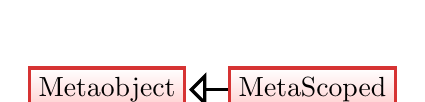
\begin{tikzpicture}
\node[concept] (Metaobject) {Metaobject};
\node[concept] (MetaScoped) [right=of Metaobject] {MetaScoped}
	edge[inheritance] (Metaobject);
\end{tikzpicture}

\meta{Scoped} is a \meta{object} reflecting program constructs defined inside
of a named scope (like the global scope, a namespace, a class, etc.)

In addition to the requirements inherited from \meta{object}, the following requirements must
be satisfied:

The \verb@has_scope@ template class specialization for a \meta{Scoped} should
inherit from \verb@true_type@:

\begin{minted}{cpp}
template <>
struct has_scope<MetaScoped>
 : true_type
{ };
\end{minted}

\subsubsection{\texttt{scope}}

A template class \verb@scope@ should be defined and should inherit from the
\meta{Scope} which reflects the parent scope of the program construct reflected
by this \meta{Scoped}.

\begin{minted}{cpp}
template <typename T>
struct scope;

template <>
struct scope<MetaScoped>
 : MetaScope
{ };
\end{minted}


\subsection{MetaNamedScoped}
\label{concept-MetaNamedScoped}

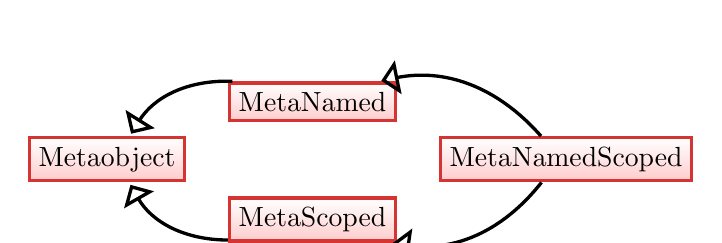
\begin{tikzpicture}
\node [concept] (Metaobject) {Metaobject};
\node [concept] (MetaNamed)[above right=of Metaobject] {MetaNamed}
	edge [inheritance, bend right] (Metaobject);
\node [concept] (MetaScoped)[below right=of Metaobject] {MetaScoped}
	edge [inheritance, bend left] (Metaobject);
\node [concept] (MetaNamedScoped)[below right=of MetaNamed, above right=of MetaScoped] {MetaNamedScoped}
	edge [inheritance, bend right] (MetaNamed)
	edge [inheritance, bend left] (MetaScoped);
\end{tikzpicture}

In addition to the requirements from \meta{Named} and \meta{Scoped},
concrete metaobjects modelling \meta{NamedScoped} must satisfy the following:

\subsubsection{\texttt{full\_name}}

A template class \verb@full_name@ should be defined an should return the fully
qualified name of the reflected construct, including the nested name specifier.

For namespace \verb@std@ the value 
should be \verb@"std"@, for namespace \verb@foo::bar::baz@ the value should
be \verb@"foo::bar::baz"@, for the global scope the value should be an empty
\concept{StringConstant}.
For \verb@std::vector<int>::iterator@ it should be \verb@"std::vector<int>::iterator"@.
For derived qualified types like
\verb@volatile std::vector<const foo::bar::fubar*> * const *@ it should be defined as
\verb@"volatile std::vector<const foo::bar::fubar*> * const *"@, etc.

\begin{lstlisting}
template <typename T>
struct full_name;

template <>
struct full_name<MetaNamedScoped>
 : StringConstant
{ };
\end{lstlisting}


\subsection{MetaScope}
\label{concept-MetaScope}

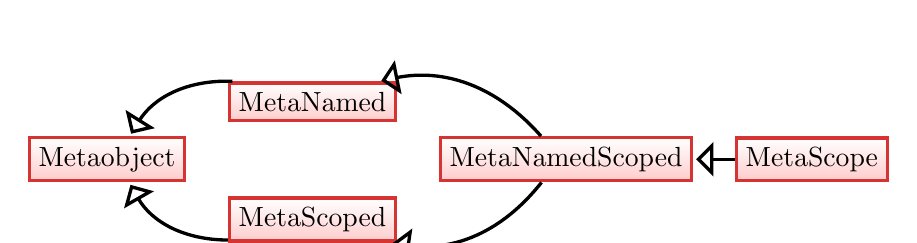
\begin{tikzpicture}
\node [concept] (Metaobject) {Metaobject};
\node [concept] (MetaNamed)[above right=of Metaobject] {MetaNamed}
	edge [inheritance, bend right] (Metaobject);
\node [concept] (MetaScoped)[below right=of Metaobject] {MetaScoped}
	edge [inheritance, bend left] (Metaobject);
\node [concept] (MetaNamedScoped)[below right=of MetaNamed, above right=of MetaScoped] {MetaNamedScoped}
	edge [inheritance, bend right] (MetaNamed)
	edge [inheritance, bend left] (MetaScoped);
\node [concept] (MetaScope)[right=of MetaNamedScoped] {MetaScope}
	edge [inheritance] (MetaNamedScoped);
\end{tikzpicture}

\meta{Scoped} is a \meta{NamedScoped} reflecting program constructs defined inside
of a named scope (like the global scope, a namespace, a class, etc.)

In addition to the requirements inherited from \meta{NamedScoped}, the following is required:

The \verb@is_scope@ template class specialization for a \meta{Scope} should
inherit from \verb@true_type@:

\begin{lstlisting}
template <>
struct is_scope<MetaScope>
 : true_type
{ };
\end{lstlisting}

\subsubsection{\texttt{members}}

A template class \verb@members@ should be defined and should inherit from a
\concept{MetaobjectSequence} containing \meta{NamedScoped} metaobjects reflecting
all members of the base-level scope reflected by this \meta{Scope}.

\begin{lstlisting}
template <typename T>
struct members;

template <>
struct members<MetaScope>
 : MetaobjectSequence<MetaNamedScoped>
{ };
\end{lstlisting}


\subsection{MetaClassMember}
\label{concept-MetaClassMember}

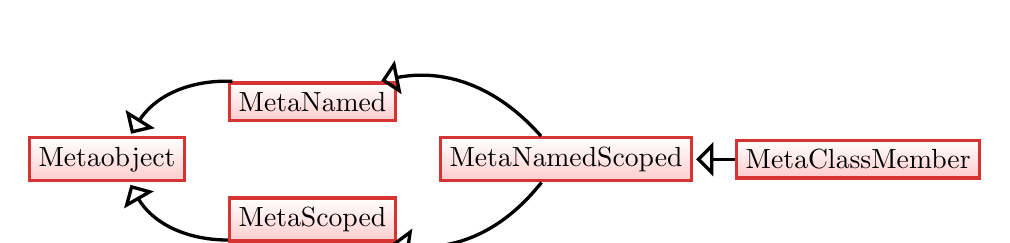
\begin{tikzpicture}
\node [concept] (Metaobject) {Metaobject};
\node [concept] (MetaNamed)[above right=of Metaobject] {MetaNamed}
	edge [inheritance, bend right] (Metaobject);
\node [concept] (MetaScoped)[below right=of Metaobject] {MetaScoped}
	edge [inheritance, bend left] (Metaobject);
\node [concept] (MetaNamedScoped)[below right=of MetaNamed, above right=of MetaScoped] {MetaNamedScoped}
	edge [inheritance, bend right] (MetaNamed)
	edge [inheritance, bend left] (MetaScoped);
\node [concept] (MetaClassMember)[right=of MetaNamedScoped] {MetaClassMember}
	edge [inheritance] (MetaNamedScoped);
\end{tikzpicture}

\meta{Class} is a \meta{Type} and a \meta{Scope} if reflecting a regular class or possibly
also a \meta{Template} if it reflects a class template.

In addition to the requirements inherited from \meta{NamedScoped},
the following is required for \meta{ClassMember}s:

The \verb@is_class_member@ template class specialization for a \meta{ClassMember} should
inherit from \verb@true_type@:

\begin{minted}{cpp}
template <>
struct is_class_member<MetaClassMember>
 : true_type
{ };
\end{minted}

\subsubsection{\texttt{access\_specifier}}

A template class called \verb@access_specifier@ should be defined and should inherit from
a \meta{Specifier} reflecting the \verb@private@, \verb@protected@ or \verb@public@
access specifier:

\begin{minted}{cpp}
template <typename T>
struct access_specifier;

template <>
struct access_specifier<MetaClassMember>
 : MetaSpecifier
{ };
\end{minted}


\subsection{MetaGlobalScope}
\label{concept-MetaGlobalScope}

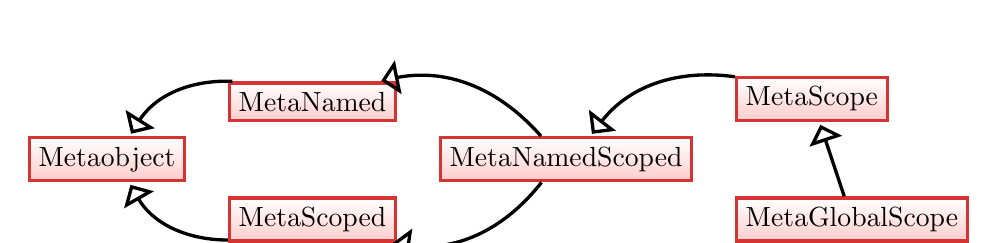
\begin{tikzpicture}
\node [concept] (Metaobject) {Metaobject};
\node [concept] (MetaNamed)[above right=of Metaobject] {MetaNamed}
	edge [inheritance, bend right] (Metaobject);
\node [concept] (MetaScoped)[below right=of Metaobject] {MetaScoped}
	edge [inheritance, bend left] (Metaobject);
\node [concept] (MetaNamedScoped)[below right=of MetaNamed, above right=of MetaScoped] {MetaNamedScoped}
	edge [inheritance, bend right] (MetaNamed)
	edge [inheritance, bend left] (MetaScoped);
\node [concept] (MetaScope)[above right=of MetaNamedScoped] {MetaScope}
	edge [inheritance, bend right] (MetaNamedScoped);
\node [concept] (MetaGlobalScope)[below right=of MetaNamedScoped] {MetaGlobalScope}
	edge [inheritance] (MetaScope);
\end{tikzpicture}

\meta{GlobalScope} is a \meta{Scope} reflecting the global scope.

In addition to the requirements inherited from \meta{Scope}, the following must
be satisfied:

The \verb@metaobject_category@ template class specialization for a \meta{GlobalScope} should
inherit from \verb@global_scope_tag@:

\begin{minted}{cpp}
template <>
struct metaobject_category<MetaNamespace>
 : global_scope_tag
{ };
\end{minted}

The \verb@scope@ template class specialization (required by \meta{Scoped}) for \meta{GlobalScope}
should inherit from the \meta{GlobalScope} itself:

\begin{minted}{cpp}
template <>
struct scope<MetaGlobalScope>
 : MetaGlobalScope
{ };
\end{minted}


\subsection{MetaNamespace}
\label{concept-MetaNamespace}

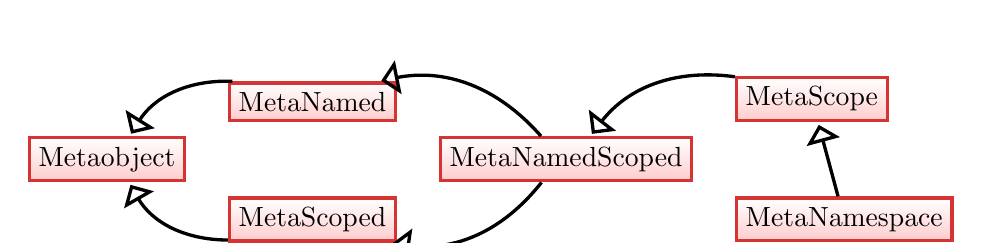
\begin{tikzpicture}
\node [concept] (Metaobject) {Metaobject};
\node [concept] (MetaNamed)[above right=of Metaobject] {MetaNamed}
	edge [inheritance, bend right] (Metaobject);
\node [concept] (MetaScoped)[below right=of Metaobject] {MetaScoped}
	edge [inheritance, bend left] (Metaobject);
\node [concept] (MetaNamedScoped)[below right=of MetaNamed, above right=of MetaScoped] {MetaNamedScoped}
	edge [inheritance, bend right] (MetaNamed)
	edge [inheritance, bend left] (MetaScoped);
\node [concept] (MetaScope)[above right=of MetaNamedScoped] {MetaScope}
	edge [inheritance, bend right] (MetaNamedScoped);
\node [concept] (MetaNamespace)[below right=of MetaNamedScoped] {MetaNamespace}
	edge [inheritance] (MetaScope);
\end{tikzpicture}

\meta{Namespace} is a \meta{Scope} reflecting a namespace.

In addition to the requirements inherited from \meta{Scope}, the following must
be satisfied:

The \verb@metaobject_category@ template class specialization for a \meta{Namespace} should
inherit from \verb@namespace_tag@:

\begin{minted}{cpp}
template <>
struct metaobject_category<MetaNamespace>
 : namespace_tag
{ };
\end{minted}


\subsection{MetaType}
\label{concept-MetaType}

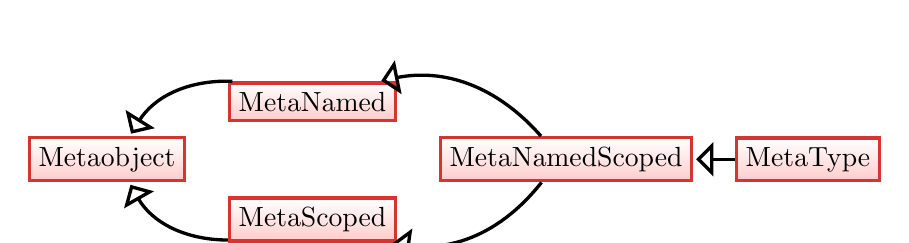
\begin{tikzpicture}
\node [concept] (Metaobject) {Metaobject};
\node [concept] (MetaNamed)[above right=of Metaobject] {MetaNamed}
	edge [inheritance, bend right] (Metaobject);
\node [concept] (MetaScoped)[below right=of Metaobject] {MetaScoped}
	edge [inheritance, bend left] (Metaobject);
\node [concept] (MetaNamedScoped)[below right=of MetaNamed, above right=of MetaScoped] {MetaNamedScoped}
	edge [inheritance, bend right] (MetaNamed)
	edge [inheritance, bend left] (MetaScoped);
\node [concept] (MetaType)[right=of MetaNamedScoped] {MetaType}
	edge [inheritance] (MetaNamedScoped);
\end{tikzpicture}

\meta{Type} is a \meta{NamedScoped} reflecting types.

In addition to the requirements inherited from \meta{NamedScoped}, the following is required:

\subsubsection{\texttt{original\_type}}

A template class \verb@original_type@ should be defined and should "return"
the original type reflected by this \meta{Type}:

\begin{lstlisting}
template <typename T>
struct original_type;

template <>
struct original_type<MetaType>
{
	typedef original-type type;
};
\end{lstlisting}

Note, that if a concept derived from \meta{Type}, for example a \meta{Class},
is also a \meta{Template} (i.e. is reflecting a template not a concrete type),
then the \verb@original_type@ template should be left undefined.


\input{sections/concepts_typedef.tex}
\input{sections/concepts_class.tex}
\subsection{MetaOverloadedFunction}
\label{concept-MetaOverloadedFunction}

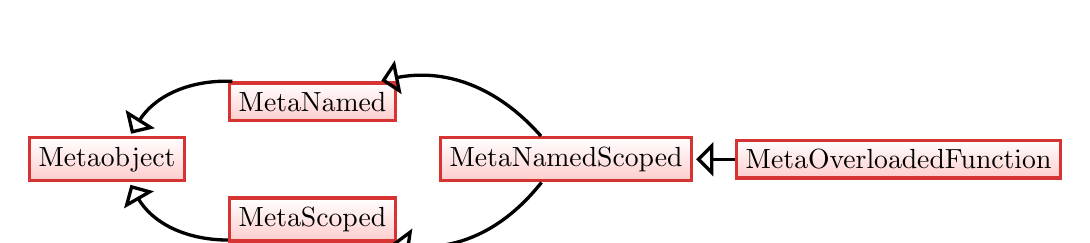
\begin{tikzpicture}
\node [concept] (Metaobject) {Metaobject};
\node [concept] (MetaNamed)[above right=of Metaobject] {MetaNamed}
	edge [inheritance, bend right] (Metaobject);
\node [concept] (MetaScoped)[below right=of Metaobject] {MetaScoped}
	edge [inheritance, bend left] (Metaobject);
\node [concept] (MetaNamedScoped)[below right=of MetaNamed, above right=of MetaScoped] {MetaNamedScoped}
	edge [inheritance, bend right] (MetaNamed)
	edge [inheritance, bend left] (MetaScoped);
\node [concept] (MetaOverloadedFunction)[right=of MetaNamedScoped] {MetaOverloadedFunction}
	edge [inheritance] (MetaNamedScoped);
\end{tikzpicture}


Models of \meta{OverloadedFunction} reflect overloaded functions.
\meta{Function}s (and \meta{Operator}s, \meta{Initializer}s, \meta{Constructor}s, etc.)
are not direct members of scopes (they are not listed in the \concept{MetaobjectSequence}
"returned" by the \verb@members<MetaScope>@ template class).
Instead, all functions, operators and constructors with the same name, (and even those that are not
overloaded in a specific scope) are grouped into a \meta{OverloadedFunction}. Individual overloaded \meta{Function}s
in the group can be obtained through the interface of \meta{OverloadedFunction} (specifically through the
\verb@overloads@ template described below). The same also applies to \meta{Constructor}s and \meta{Operator}s.

The rationale for this is that direct scope members, i.e. metaobjects accessible through the \meta{Scope}'s
\verb@members@ template class should have unique names, which would not be the case if \meta{Function}s
were direct scope members.

The \verb@scope@ of an \meta{OverloadedFunction} is the same as the \verb@scope@
of all \meta{Function}s grouped by that \meta{OverloadedFunction}.

In addition to the requirements inherited from \meta{NamedScoped},
models of \meta{OverloadedFunction} are subject to the following:

The \verb@metaobject_category@ template class specialization for a \meta{OverloadedFunction}
should inherit from \verb@overloaded_function_tag@:

\begin{minted}{cpp}
template <>
struct metaobject_category<MetaOverloadedFunction>
 : overloaded_function_tag
{ };
\end{minted}

\subsubsection{\texttt{overloads}}

A template class called \verb@overloads@ should be defined and should
return a \concept{MetaobjectSequence} of \meta{Function}s, reflecting
the individual overloads:

\begin{minted}{cpp}
template <>
struct overloads<MetaOverloadedFunction>
 : MetaobjectSequence<MetaFunction>
{ };
\end{minted}


\subsection{MetaFunction}
\label{concept-MetaFunction}

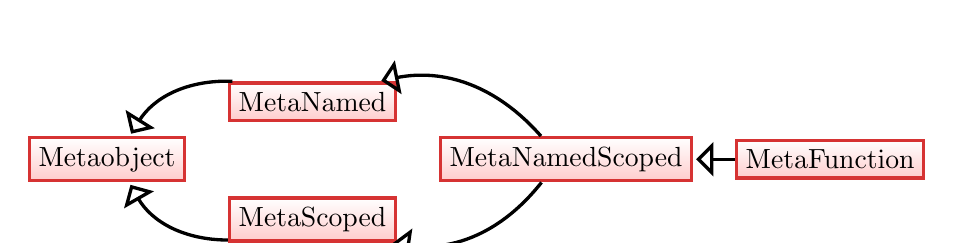
\begin{tikzpicture}
\node [concept] (Metaobject) {Metaobject};
\node [concept] (MetaNamed)[above right=of Metaobject] {MetaNamed}
	edge [inheritance, bend right] (Metaobject);
\node [concept] (MetaScoped)[below right=of Metaobject] {MetaScoped}
	edge [inheritance, bend left] (Metaobject);
\node [concept] (MetaNamedScoped)[below right=of MetaNamed, above right=of MetaScoped] {MetaNamedScoped}
	edge [inheritance, bend right] (MetaNamed)
	edge [inheritance, bend left] (MetaScoped);
\node [concept] (MetaFunction)[right=of MetaNamedScoped] {MetaFunction}
	edge [inheritance] (MetaNamedScoped);
\end{tikzpicture}


\meta{Function} reflects a function or function template.
\meta{Function}s are not direct members of scopes (they are not listed in the \concept{MetaobjectSequence}
"returned" by the \verb@members<MetaScope>@ template class).
Instead, all functions with the same name, (and even those that are not
overloaded in a specific scope) are grouped into a \meta{OverloadedFunction}. Individual overloaded \meta{Function}s
in the group can be obtained through the interface of \meta{OverloadedFunction} (specifically through the
\verb@overloads@ template described below). The same also applies to \meta{Constructor}s and \meta{Operator}s.

The rationale for this is that direct scope members, i.e. metaobjects accessible through the \meta{Scope}'s
\verb@members@ template class should have unique names, which would not be the case if \meta{Function}s
were direct scope members.

The \verb@scope@ of an \meta{OverloadedFunction} is the same as the \verb@scope@
of all \meta{Function}s grouped by that \meta{OverloadedFunction}.

In addition to the requirements inherited from \meta{NamedScoped},
models of \meta{Function} are subject to the following:

The \verb@metaobject_category@ template class specialization for a \meta{Function} should
inherit from \verb@function_tag@:

\begin{minted}{cpp}
template <>
struct metaobject_category<MetaFunction>
 : function_tag
{ };
\end{minted}

If a \meta{Function} reflects a function template, then the \verb@is_template@
trait should inherit from \verb@true_type@

\subsubsection{\texttt{linkage\_specifier}}

A template class \verb@linkage_specifier@ should be defined and should inherit from
a \meta{Specifier} reflecting the linkage specifier of the function reflected by
the \meta{Function}:

\begin{minted}{cpp}
template <typename T>
struct linkage_specifier;

template <>
struct linkage_specifier<MetaFunction>
 : MetaSpecifier
{ };
\end{minted}

\subsubsection{\texttt{constexpr\_specifier}}

A template class \verb@constexpr_specifier@ should be defined and should inherit from
a \meta{Specifier} reflecting the constexpr specifier of the reflected function:

\begin{minted}{cpp}
template <typename T>
struct constexpr_specifier;

template <>
struct constexpr_specifier<MetaFunction>
 : MetaSpecifier
{ };
\end{minted}

In case the reflected function does not have the \verb@constexpr@ specifier,
then the result should be a \meta{Specifier} reflecting the "none" specifier.

\subsubsection{\texttt{result\_type}}

A template class \verb@result_type@ should be defined and should inherit from
a \meta{Type} reflecting the return value type of the reflected function:

\begin{minted}{cpp}
template <typename T>
struct result_type;

template <>
struct result_type<MetaFunction>
 : MetaType
{ };
\end{minted}

\subsubsection{\texttt{parameters}}

A template class \verb@parameters@ should be defined and should inherit from
a \concept{MetaobjectRange} or \meta{Parameter}s reflecting the individual parameters
of the function:

\begin{minted}{cpp}
template <typename T>
struct parameters;

template <>
struct parameters<MetaFunction>
 : MetaobjectRange<MetaParameter>
{ };
\end{minted}

\subsubsection{\texttt{noexcept\_specifier}}

A template class \verb@noexcept_specifier@ should be defined and should inherit from
a \meta{Specifier} reflecting the noexcept specifier of the reflected function:

\begin{minted}{cpp}
template <typename T>
struct noexcept_specifier;

template <>
struct noexcept_specifier<MetaFunction>
 : MetaSpecifier
{ };
\end{minted}

In case the reflected function does not have the \verb@noexcept@ specifier,
then the result should be a \meta{Specifier} reflecting the "none" specifier.

\subsubsection{\texttt{exceptions}}

A template class \verb@exceptions@ should be defined and should inherit from
a \concept{MetaobjectRange} of \meta{Type}s reflecting the individual exception types
that the reflected function is allowed to throw:

\begin{minted}{cpp}
template <typename T>
struct exceptions;

template <>
struct exceptions<MetaFunction>
 : MetaobjectRange<MetaType>
{ };
\end{minted}

\subsubsection{\texttt{const\_specifier}}

In case a \meta{Function} is also a \meta{ClassMember},
a template class \verb@const_specifier@ should be defined and should inherit from
a \meta{Specifier} reflecting the const specifier of the reflected member function:

\begin{minted}{cpp}
template <typename T>
struct const_specifier;

template <>
struct const_specifier<MetaFunction>
 : MetaSpecifier
{
	static_assert(is_class_member<MetaFunction>::value, "");
};
\end{minted}

In case the reflected member function does not have the \verb@const@ specifier,
then the result should be a \meta{Specifier} reflecting the "none" specifier.

\subsubsection{\texttt{pure\_virtual}}

In case a \meta{Function} is also a \meta{ClassMember},
a template class \verb@pure_virtual@ should be defined and should inherit from
\verb@true_type@ if the reflected function is pure virtual or from \verb@false_type@
otherwise:

\begin{minted}{cpp}
template <typename T>
struct pure_virtual;

struct pure_virtual<MetaFunction>
 : std::integral_constant<bool, B>
{
	static_assert(is_class_member<MetaFunction>::value, "");
};
\end{minted}


\subsection{MetaInitializer}
\label{concept-MetaInitializer}

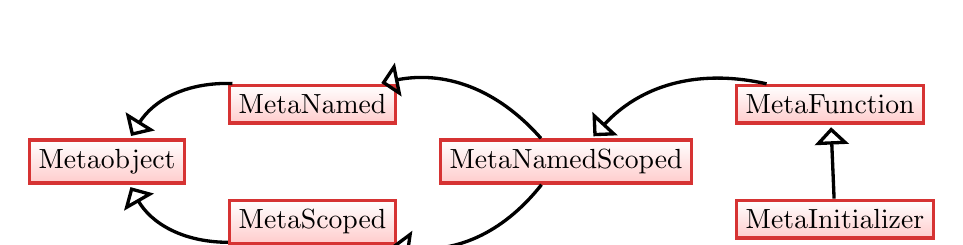
\begin{tikzpicture}
\node [concept] (Metaobject) {Metaobject};
\node [concept] (MetaNamed)[above right=of Metaobject] {MetaNamed}
	edge [inheritance, bend right] (Metaobject);
\node [concept] (MetaScoped)[below right=of Metaobject] {MetaScoped}
	edge [inheritance, bend left] (Metaobject);
\node [concept] (MetaNamedScoped)[below right=of MetaNamed, above right=of MetaScoped] {MetaNamedScoped}
	edge [inheritance, bend right] (MetaNamed)
	edge [inheritance, bend left] (MetaScoped);
\node [concept] (MetaFunction)[above right=of MetaNamedScoped] {MetaFunction}
	edge [inheritance, bend right] (MetaNamedScoped);
\node [concept] (MetaInitializer)[below right=of MetaNamedScoped] {MetaInitializer}
	edge [inheritance] (MetaFunction);
\end{tikzpicture}


\meta{Initializer} reflects an initializer (constructor) of a native type.

In addition to the requirements inherited from \meta{Function},
models of \meta{Initializer} must conform to the following:

The \verb@metaobject_category@ template class specialization for a \meta{Initializer} should
inherit from \verb@constructor_tag@:

\begin{minted}{cpp}
template <>
struct metaobject_category<MetaInitializer>
 : constructor_tag
{ };
\end{minted}

The specialization of the \verb@result_type@ template class for a \meta{Initializer} should
inherit from a \meta{Type} reflecting the initialized type:

\begin{minted}{cpp}
template <>
struct result_type<MetaInitializer>
 : MetaType
{ };
\end{minted}


\subsection{MetaConstructor}
\label{concept-MetaConstructor}

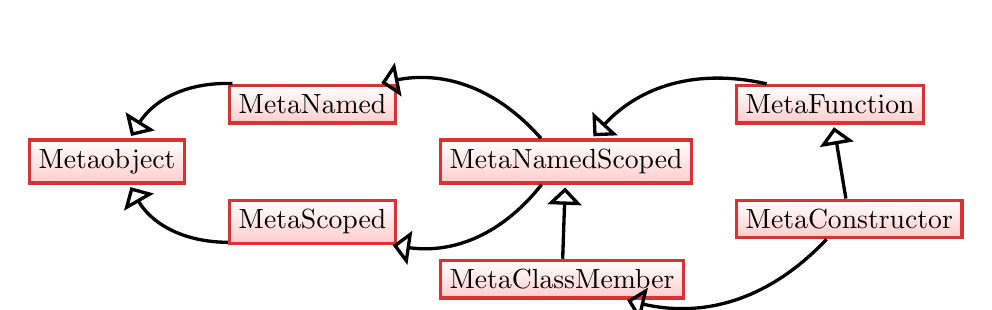
\begin{tikzpicture}
\node [concept] (Metaobject) {Metaobject};
\node [concept] (MetaNamed)[above right=of Metaobject] {MetaNamed}
	edge [inheritance, bend right] (Metaobject);
\node [concept] (MetaScoped)[below right=of Metaobject] {MetaScoped}
	edge [inheritance, bend left] (Metaobject);
\node [concept] (MetaNamedScoped)[below right=of MetaNamed, above right=of MetaScoped] {MetaNamedScoped}
	edge [inheritance, bend right] (MetaNamed)
	edge [inheritance, bend left] (MetaScoped);
\node [concept] (MetaFunction)[above right=of MetaNamedScoped] {MetaFunction}
	edge [inheritance, bend right] (MetaNamedScoped);
\node [concept] (MetaClassMember)[below right=of MetaScoped] {MetaClassMember}
	edge [inheritance] (MetaNamedScoped);
\node [concept] (MetaConstructor)[below right=of MetaNamedScoped] {MetaConstructor}
	edge [inheritance] (MetaFunction)
	edge [inheritance, bend left] (MetaClassMember);
\end{tikzpicture}


\meta{Constructor} reflects a constructor of an elaborated type.

In addition to the requirements inherited from \meta{Function} and \meta{ClassMember},
the following is required for \meta{Constructor}s:

The \verb@metaobject_category@ template class specialization for a \meta{Constructor} should
inherit from \verb@constructor_tag@:

\begin{minted}{cpp}
template <>
struct metaobject_category<MetaConstructor>
 : constructor_tag
{ };
\end{minted}

The specialization of the \verb@result_type@ template class for a \meta{Constructor} should
inherit from a \meta{Class} reflecting the constructed type.

\begin{minted}{cpp}
template <>
struct result_type<MetaConstructor>
 : MetaClass
{ };
\end{minted}

The specialization of the \verb@scope@ template class for a \meta{Constructor} should
inherit from a \meta{Class} reflecting the constructed type.

\begin{minted}{cpp}
template <>
struct scope<MetaConstructor>
 : MetaClass
{ };
\end{minted}


\subsection{MetaOperator}
\label{concept-MetaOperator}

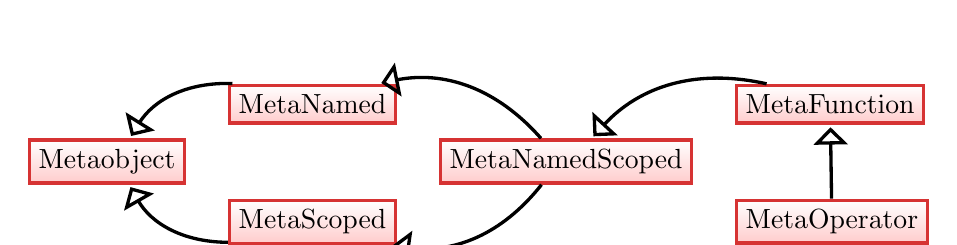
\begin{tikzpicture}
\node [concept] (Metaobject) {Metaobject};
\node [concept] (MetaNamed)[above right=of Metaobject] {MetaNamed}
	edge [inheritance, bend right] (Metaobject);
\node [concept] (MetaScoped)[below right=of Metaobject] {MetaScoped}
	edge [inheritance, bend left] (Metaobject);
\node [concept] (MetaNamedScoped)[below right=of MetaNamed, above right=of MetaScoped] {MetaNamedScoped}
	edge [inheritance, bend right] (MetaNamed)
	edge [inheritance, bend left] (MetaScoped);
\node [concept] (MetaFunction)[above right=of MetaNamedScoped] {MetaFunction}
	edge [inheritance, bend right] (MetaNamedScoped);
\node [concept] (MetaOperator)[below right=of MetaNamedScoped] {MetaOperator}
	edge [inheritance] (MetaFunction);
\end{tikzpicture}


\meta{Operator} is a \meta{Function} which reflects an operator.

In addition to the requirements inherited from \meta{Function},
models of \meta{Operator} must conform to the following:

The \verb@metaobject_category@ template class specialization for a \meta{Operator} should
inherit from \verb@operator_tag@:

\begin{minted}{cpp}
template <>
struct metaobject_category<MetaOperator>
 : operator_tag
{ };
\end{minted}


\input{sections/concepts_template.tex}
\subsection{MetaTemplateParameter}
\label{concept-MetaTemplateParameter}

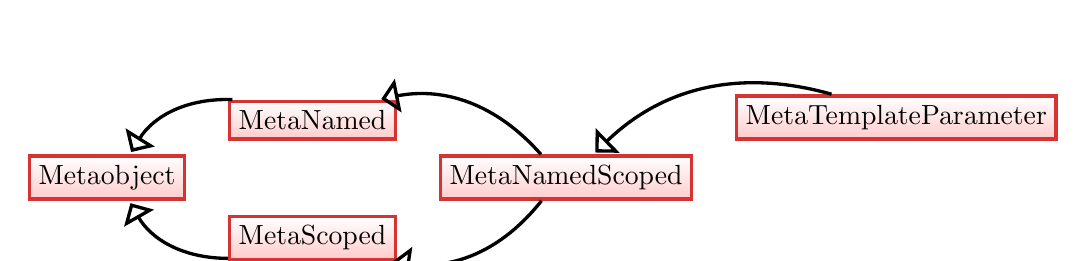
\begin{tikzpicture}
\node [concept] (Metaobject) {Metaobject};
\node [concept] (MetaNamed)[above right=of Metaobject] {MetaNamed}
	edge [inheritance, bend right] (Metaobject);
\node [concept] (MetaScoped)[below right=of Metaobject] {MetaScoped}
	edge [inheritance, bend left] (Metaobject);
\node [concept] (MetaNamedScoped)[below right=of MetaNamed, above right=of MetaScoped] {MetaNamedScoped}
	edge [inheritance, bend right] (MetaNamed)
	edge [inheritance, bend left] (MetaScoped);
\node [concept] (MetaTemplateParameter)[above right=of MetaNamedScoped] {MetaTemplateParameter}
	edge [inheritance, bend right] (MetaNamedScoped);
\end{tikzpicture}


\meta{TemplateParameter} is a \meta{NamedScoped} and either a \meta{Typedef} or a \meta{Constant}.

In addition to the requirements inherited from \meta{NamedScoped},
models of \meta{TemplateParameter} must conform to the following:

The \verb@is_template@ template class specialization for a \meta{TemplateParameter} should
inherit from \verb@true_type@:

\begin{minted}{cpp}
template <>
struct is_template<MetaTemplateParameter>
 : true_type
{ };
\end{minted}

The \verb@full_name@ inherited from \meta{Named} should return the same \concept{StringConstant}
as \verb@base_name@ for models of \meta{TemplateParameter}, i.e. the plain template parameter
name without any qualifications.

\subsubsection{\texttt{position}}

A template class \verb@position@ should be defined and should
inherit from \verb@integral_constant<size_t, I>@ where \verb@I@ is
a zero-based position (index) of the parameter.

\begin{minted}{cpp}
template <typename T>
struct position;

template <>
struct position<MetaTemplateParameter>
 : integral_constant<size_t, I>
{ };
\end{minted}

\subsubsection{\texttt{is\_pack}}

A template class called \verb@is_pack@ should be defined and should
inherit from \verb@true_type@ if the template parameter is a pack
parameter or from \verb@false_type@ otherwise.

\begin{minted}{cpp}
template <typename T>
struct is_pack;

template <>
struct is_pack<MetaTemplateParameter>
 : integral_constant<bool, B>
{ };
\end{minted}


\input{sections/concepts_instantiation.tex}
\subsection{MetaEnum}
\label{concept-MetaEnum}

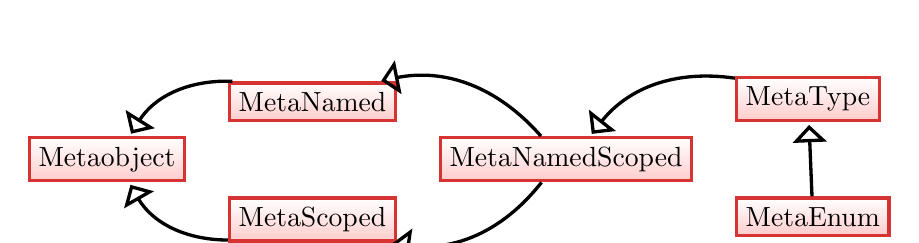
\begin{tikzpicture}
\node [concept] (Metaobject) {Metaobject};
\node [concept] (MetaNamed)[above right=of Metaobject] {MetaNamed}
	edge [inheritance, bend right] (Metaobject);
\node [concept] (MetaScoped)[below right=of Metaobject] {MetaScoped}
	edge [inheritance, bend left] (Metaobject);
\node [concept] (MetaNamedScoped)[below right=of MetaNamed, above right=of MetaScoped] {MetaNamedScoped}
	edge [inheritance, bend right] (MetaNamed)
	edge [inheritance, bend left] (MetaScoped);
\node [concept] (MetaType)[above right=of MetaNamedScoped] {MetaType}
	edge [inheritance, bend right] (MetaNamedScoped);
\node [concept] (MetaEnum)[below right=of MetaNamedScoped] {MetaEnum}
	edge [inheritance] (MetaType);
\end{tikzpicture}

\meta{Enum} is a \meta{Type} reflecting an enumeration type.

In addition to the requirements inherited from \meta{Type}, \meta{Enum} requires
also the following:

The \verb@metaobject_category@ template class specialization for a \meta{Enum} should
inherit from \verb@enum_tag@:

\begin{minted}{cpp}
template <>
struct metaobject_category<MetaEnum>
 : enum_tag
{ };
\end{minted}

The \verb@members@ of \meta{EnumClass} are only \meta{Named} \meta{Constant}s.

\subsubsection{\texttt{base\_type}}

A template class \verb@base_type@ should be defined and should inherit from
a \meta{Type} reflecting the underlying type of the enumeration:

\begin{minted}{cpp}
template <typename T>
struct base_type;

template <>
struct base_type<MetaEnum>
 : MetaType
{ };
\end{minted}

\subsection{MetaEnumClass}
\label{concept-MetaEnumClass}

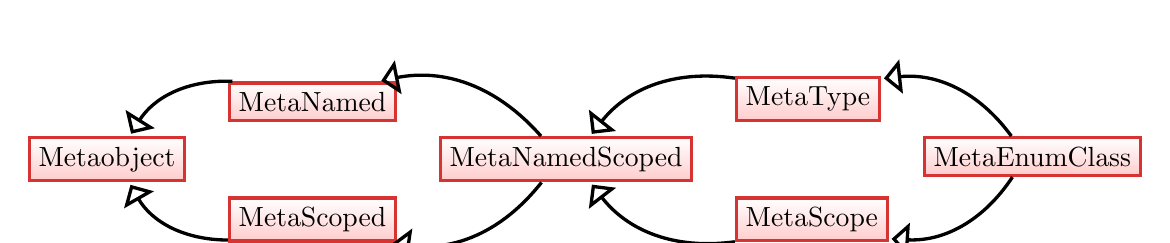
\begin{tikzpicture}
\node [concept] (Metaobject) {Metaobject};
\node [concept] (MetaNamed)[above right=of Metaobject] {MetaNamed}
	edge [inheritance, bend right] (Metaobject);
\node [concept] (MetaScoped)[below right=of Metaobject] {MetaScoped}
	edge [inheritance, bend left] (Metaobject);
\node [concept] (MetaNamedScoped)[below right=of MetaNamed, above right=of MetaScoped] {MetaNamedScoped}
	edge [inheritance, bend right] (MetaNamed)
	edge [inheritance, bend left] (MetaScoped);
\node [concept] (MetaType)[above right=of MetaNamedScoped] {MetaType}
	edge [inheritance, bend right] (MetaNamedScoped);
\node [concept] (MetaScope)[below right=of MetaNamedScoped] {MetaScope}
	edge [inheritance, bend left] (MetaNamedScoped);
\node [concept] (MetaEnumClass)[below right=of MetaType] {MetaEnumClass}
	edge [inheritance, bend right] (MetaType)
	edge [inheritance, bend left] (MetaScope);
\end{tikzpicture}

\meta{EnumClass} is a \meta{Type} and a \meta{Scope} reflecting a strongly type enumeration.

In addition to the requirements inherited from \meta{Type} and \meta{Scope}, the following must
be satisfied:

The \verb@metaobject_category@ template class specialization for a \meta{EnumClass} should
inherit from \verb@enum_class@:

\begin{minted}{cpp}
template <>
struct metaobject_category<MetaEnumClass>
 : enum_class_tag
{ };
\end{minted}

The \verb@members@ of \meta{EnumClass} are only \meta{NamedScoped} \meta{Constants}.

\subsubsection{\texttt{base\_type}}

A template class \verb@base_type@ should be defined and should inherit from
a \meta{Type} reflecting the base type of the enumeration:

\begin{minted}{cpp}
template <typename T>
struct base_type;

template <>
struct base_type<MetaEnumClass>
 : MetaType
{ };
\end{minted}

\subsection{MetaInheritance}
\label{concept-MetaInheritance}

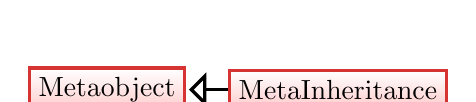
\begin{tikzpicture}
\node[concept] (Metaobject) {Metaobject};
\node[concept] (MetaInheritance) [right=of Metaobject] {MetaInheritance}
	edge[inheritance] (Metaobject);
\end{tikzpicture}

\meta{Inheritance} is a \meta{object} reflecting class inheritance.

In addition to the requirements inherited from \meta{object}, types conforming to this concept
must satisfy the following:

The \verb@metaobject_category@ template should return \verb@inheritance_tag@ for models
of \meta{Inheritance}.

\begin{minted}{cpp}
template <>
struct metaobject_category<MetaInheritance>
 : inheritance_tag
{ };
\end{minted}

\subsubsection{\texttt{access\_specifier}}

A template struct \verb@access_specifier@ should be defined and should inherit from
a \meta{Specifier} reflecting one of the \verb@private@, \verb@protected@ and
\verb@public@ access specifiers.

\begin{minted}{cpp}
template <typename T>
struct access_specifier;

template <>
struct access_specifier<MetaInheritance>
 : MetaSpecifier
{ };
\end{minted}

\subsubsection{\texttt{inheritance\_specifier}}

A template struct \verb@inheritance_specifier@ should be defined and should inherit from
a \meta{Specifier} reflecting one of the \verb@virtual@ and "none" access specifiers.

\begin{minted}{cpp}
template <typename T>
struct inheritance_specifier;

template <>
struct inheritance_specifier<MetaInheritance>
 : MetaSpecifier
{ };
\end{minted}

\subsubsection{\texttt{base\_class}}

A template struct \verb@base_class@ should be defined and should inherit from
a \meta{Class} reflecting the base class in the inheritance:

\begin{minted}{cpp}
template <typename T>
struct base_class;

template <>
struct base_class<MetaInheritance>
 : MetaClass
{ };
\end{minted}

\subsubsection{\texttt{derived\_class}}

A template struct \verb@derived_class@ should be defined and should inherit from
a \meta{Class} reflecting the derived class in the inheritance:

\begin{minted}{cpp}
template <typename T>
struct derived_class;

template <>
struct derived_class<MetaInheritance>
 : MetaClass
{ };
\end{minted}


\subsection{MetaVariable}
\label{concept-MetaVariable}

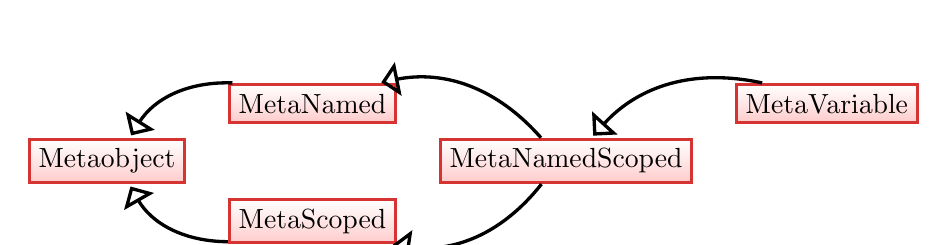
\begin{tikzpicture}
\node [concept] (Metaobject) {Metaobject};
\node [concept] (MetaNamed)[above right=of Metaobject] {MetaNamed}
	edge [inheritance, bend right] (Metaobject);
\node [concept] (MetaScoped)[below right=of Metaobject] {MetaScoped}
	edge [inheritance, bend left] (Metaobject);
\node [concept] (MetaNamedScoped)[below right=of MetaNamed, above right=of MetaScoped] {MetaNamedScoped}
	edge [inheritance, bend right] (MetaNamed)
	edge [inheritance, bend left] (MetaScoped);
\node [concept] (MetaVariable)[above right=of MetaNamedScoped] {MetaVariable}
	edge [inheritance, bend right] (MetaNamedScoped);
\end{tikzpicture}

\meta{Variable} is a \meta{NamedScoped} reflecting a variable.

In addition to the requirements inherited from \meta{NamedScoped}, the following must
be satisfied:

The \verb@metaobject_category@ template class specialization for a \meta{Variable} should
inherit from \verb@variable_tag@:

\begin{minted}{cpp}
template <>
struct metaobject_category<MetaVariable>
 : variable_tag
{ };
\end{minted}

\subsubsection{\texttt{storage\_specifier}}

A template class \verb@storage_specifier@ should be added and should
inherit from a \meta{Specifier} reflecting a storage class specifier:

\begin{minted}{cpp}
template <typename T>
struct storage_specifier;

template <>
struct storage_specifier<MetaVariable>
 : MetaSpecifier
{ };
\end{minted}

\subsubsection{\texttt{type}}

A template class \verb@type@ should be added and should inherit
from a \meta{Type} reflecting the type of the variable:

\begin{minted}{cpp}
template <typename T>
struct type;

template <>
struct type<MetaVariable>
 : MetaType
{ };
\end{minted}

\subsubsection{\texttt{pointer}}

If the reflected variable is a namespace-level variable, then a template
class \verb@pointer@ should be implemented as follows:

\begin{minted}{cpp}
template <typename T>
struct pointer;

template <>
struct pointer<MetaVariable>
{
	typedef typename original_type<type<MetaVariable>>::type* type;

	static type get(void);
};
\end{minted}

The static member function \verb@get@ should return the address of the reflected variable.

If the reflected variable is a class member variable (i.e. if the \meta{Variable}
is also a \meta{ClassMember}), then the \verb@pointer@ template class should be
defined as follows:

\begin{minted}{cpp}

template <>
struct pointer<MetaVariable>
{
	typedef typename original_type<type<MetaVariable>>::type
		_mv_t;
	typedef typename original_type<type<scope<MetaVariable>>>::type
		_cls_t;

	typedef _mv_t _cls_t::* type;

	static type get(void);
};

\end{minted}

The static member function \verb@get@ should return a data member pointer to
the reflected member variable. The \verb@_mv_t@ and \verb@_cls_t@ typedefs
are implementation details and are not a part of this specification.

\subsection{MetaParameter}
\label{concept-MetaParameter}

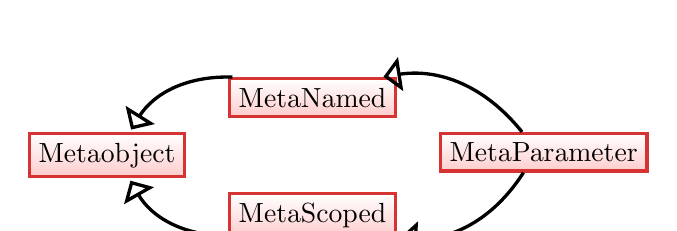
\begin{tikzpicture}
\node [concept] (Metaobject) {Metaobject};
\node [concept] (MetaNamed)[above right=of Metaobject] {MetaNamed}
	edge [inheritance, bend right] (Metaobject);
\node [concept] (MetaScoped)[below right=of Metaobject] {MetaScoped}
	edge [inheritance, bend left] (Metaobject);
\node [concept] (MetaParameter)[below right=of MetaNamed] {MetaParameter}
	edge [inheritance, bend right] (MetaNamed)
	edge [inheritance, bend left] (MetaScoped);
\end{tikzpicture}

\meta{Parameter} is a \meta{Named} and \meta{Scoped},
reflecting a function parameter or a parameter pack.

In addition to the requirements inherited from \meta{Named} and \meta{Scoped},
the following must be satisfied:

The \verb@metaobject_category@ template class specialization for a \meta{Parameter} should
inherit from \verb@parameter_tag@:

\begin{minted}{cpp}
template <>
struct metaobject_category<MetaParameter>
 : parameter_tag
{ };
\end{minted}

The \verb@scope@ of a \meta{Parameter} should be a \meta{Function} reflecting
the function to which the parameter belongs:

\begin{minted}{cpp}
template <>
struct scope<MetaParameter>
 : MetaFunction
{ };
\end{minted}

The \verb@full_name@ inherited from \meta{Named} should return the same \concept{StringConstant}
as \verb@base_name@ for models of \meta{Parameter}, i.e. the plain parameter
name without any qualifications.

\subsubsection{\texttt{type}}

A template class \verb@type@ should be added and should inherit
from a \meta{Type} reflecting the type of the parameter:

\begin{minted}{cpp}
template <typename T>
struct type;

template <>
struct type<MetaParameter>
 : MetaType
{ };
\end{minted}

\subsubsection{\texttt{position}}

A template class \verb@position@ should be defined and should
inherit from \verb@integral_constant<size_t, I>@ type where \verb@I@ is
a zero-based position (index) of the parameter.

\begin{minted}{cpp}
template <typename T>
struct position;

template <>
struct position<MetaParameter>
 : integral_constant<size_t, I>
{ };
\end{minted}

\subsubsection{\texttt{is\_pack}}

A template class called \verb@is_pack@ should be defined and should
inherit from \verb@true_type@ if the parameter is a pack
parameter or from \verb@false_type@ otherwise.

\begin{minted}{cpp}
template <typename T>
struct is_pack;

template <>
struct is_pack<MetaParameter>
 : integral_constant<bool, B>
{ };
\end{minted}


\subsection{MetaConstant}
\label{concept-MetaConstant}

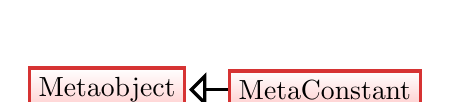
\begin{tikzpicture}
\node [concept] (Metaobject) {Metaobject};
\node [concept] (MetaConstant)[right=of Metaobject] {MetaConstant}
	edge [inheritance] (Metaobject);
\end{tikzpicture}

\meta{Constant} is a \meta{object} reflecting a compile-time constant value.

In addition to the requirements inherited from \meta{object}, the following must
be satisfied:

The \verb@metaobject_category@ template class specialization for a \meta{Constant} should
inherit from \verb@constant_tag@:

\begin{minted}{cpp}
template <>
struct metaobject_category<MetaConstant>
 : constant_tag
{ };
\end{minted}

\subsubsection{\texttt{type}}

A template class \verb@type@ should be added and should inherit
from a \meta{Type} reflecting the type of the constant value

\begin{minted}{cpp}
template <typename T>
struct type;

template <>
struct type<MetaVariable>
 : MetaType
{ };
\end{minted}

\subsubsection{\texttt{value}}

A template class \verb@value@ should be added and should inherit
from an \verb@integral_constant<T, V>@:

\begin{minted}{cpp}
template <typename T>
struct value;

template <>
struct value<MetaConstant>
 : integral_constant<T, V>
{ };
\end{minted}



\section{Reflection operator}

The metaobjects reflecting some program feature \verb@X@ as
described above should be made available to the user by
the means of a new operator or expression.
More precisely, the reflection operator returns a type conforming to a particular
metaobject concept, depending on the reflected expression.

Since adding a new keyword has the potential to break existing code,
we do not insist on any particular expression, here follows a list of suggestions
in order of preference (from the most to the least preferrable):

\begin{itemize}
\item{\verb@mirrored(X)@}
\item{\verb@reflected(X)@}
\item{\verb@reflexpr(X)@}
\item{\verb@|X@}
\item{\verb@[[X]]@}
\item{\verb@<<X>>@}
\end{itemize}

The reflected expression \verb@X@ in the items listed above can be any of the following:

\begin{itemize}
\item{\verb@::@} -- The global scope, the returned metaobject is a {\meta{GlobalScope}}.
\item{{\em Namespace name}} -- (\verb@std@) the returned metaobject is a {\meta{Namespace}}.
\item{{\em Type name}} -- (\verb@long double@) the returned metaobject is a {\meta{Type}}.
\item{{\em \verb@typedef@ name}} -- (\verb@std::size_t@ or \verb@std::string@)
     the returned metaobject is a {\meta{Typedef}}.
\item{{\em Template name}} -- (\verb@std::tuple@ or \verb@std::map@)
     the returned metaobject is a {\meta{Template}}.
\item{{\em Class name}} -- (\verb@std::thread@ or \verb@std::map<int, double>@)
     the returned metaobject is a {\meta{Class}}.
\item{{\em Function name}} -- (\verb@std::sin@ or \verb@std::string::size@) the returned metaobject
     is a {\meta{OverloadedFunction}}.
\item{{\em Function signature}} -- (\verb@std::sin(double)@ or \verb@std::string::front(void) const@)
     the returned metaobject is a {\meta{Function}}. The signature may be specified without the
     return value type.
\item{{\em Constructor signature}} -- (\verb@std::pair<char, double>::pair(char, double)@
     or \verb@std::string::string(void)@) the returned metaobject is a {\meta{Constructor}}.
\item{{\em Variable name}} -- (\verb@std::errno@) the returned metaobject is a {\meta{Variable}}.
\item{TODO}
\end{itemize}


\section{Examples}

This section contains multiple examples of usage of the additions proposed above.
The examples assume that the \verb@mirrored@ operator (described above) is used
to obtain the metaobjects and the types, templates, etc. are defined in the
\verb@std::meta@ namespace.

For the sake of brevity

\begin{minted}{cpp}
using namespace std;
\end{minted}

is assumed.

\begin{minted}[tabsize=4]{cpp}
static_assert(not(is_metaobject<int>()), "");
static_assert(not(is_metaobject<std::string>()), "");
static_assert(not(is_metaobject<my_class>()), "");

// reflected global scope
typedef mirrored(::) meta_gs;

static_assert(is_metaobject<meta_gs>(), "");

static_assert(meta::has_name<meta_gs>(), "");
static_assert(meta::has_scope<meta_gs>(), "");

static_assert(
	is_base_of<
		meta::global_scope_tag,
		meta::metaobject_category<meta_gs>
	>(), ""
);


\end{minted}

TODO



\section{Acknowledgements}

Thanks to Chandler Carruth for presenting the N4111 proposal at the Urbana meeting.
Also thanks to Axel Naumann for helping with this proposal.


\renewcommand\refname{\arabic{section}\hspace{1em}References}

\stepcounter{section}
\addcontentsline{toc}{section}{\refname}

\begin{thebibliography}{100}

\bibitem{mirror-doc-cpp11}
Mirror C++ reflection utilities (C++11 version),
\url{http://kifri.fri.uniza.sk/~chochlik/mirror-lib/html/}.

\bibitem{mirror-doc-mirror-examples}
Mirror - Examples of usage,
\url{http://kifri.fri.uniza.sk/~chochlik/mirror-lib/html/doxygen/mirror/html/examples.html}.

\bibitem{mirror-doc-puddle-examples}
Mirror - The Puddle layer - examples of usage,
\url{http://kifri.fri.uniza.sk/~chochlik/mirror-lib/html/doxygen/puddle/html/examples.html}.

\bibitem{mirror-doc-rubber-examples}
Mirror - The Rubber layer - examples of usage,
\url{http://kifri.fri.uniza.sk/~chochlik/mirror-lib/html/doxygen/rubber/html/examples.html}.

\bibitem{mirror-doc-lagoon-examples}
Mirror - The Lagoon layer - examples of usage,
\url{http://kifri.fri.uniza.sk/~chochlik/mirror-lib/html/doxygen/lagoon/html/examples.html}.

\bibitem{mirror-ct-strings}
Mirror - Compile-time strings
\url{http://kifri.fri.uniza.sk/~chochlik/mirror-lib/html/doxygen/mirror/html/d5/d1d/group__ct__string.html}.


\end{thebibliography}



%\appendix
%\section{Concept hierarchy}
\label{appendix-concept-hierarchy}

\subsection{String}

\begin{minted}{cpp}
class String
{
public:
	static constexpr const char* c_str(void);

	static constexpr size_t size(void);	
};

static_assert(
	String::c_str() != nullptr,
	"Undefined string"
);
\end{minted}

\subsection{MetaobjectCategory}

\begin{minted}{cpp}
struct metaobject_tag
{ };

struct specifier_tag
 : metaobject_tag
{ };

struct spec_extern_tag
 : specifier_tag
{ };

struct spec_static_tag
 : specifier_tag
{ };

struct spec_mutable_tag
 : specifier_tag
{ };

struct spec_register_tag
 : specifier_tag
{ };

struct spec_thread_local_tag
 : specifier_tag
{ };

struct spec_thread_local_tag
 : specifier_tag
{ };

struct spec_const_tag
 : specifier_tag
{ };

struct spec_virtual_tag
 : specifier_tag
{ };

struct spec_private_tag
 : specifier_tag
{ };

struct spec_protected_tag
 : specifier_tag
{ };

struct spec_public_tag
 : specifier_tag
{ };

struct spec_class_tag
 : specifier_tag
{ };

struct spec_struct_tag
 : specifier_tag
{ };

struct spec_union_tag
 : specifier_tag
{ };

struct spec_enum_tag
 : specifier_tag
{ };

struct namespace_tag
{ };

struct global_scope_tag
{ };

struct type_tag
{ };

struct typedef_tag
{ };

struct class_tag
{ };

struct function_tag
{ };

struct constructor_tag
{ };

struct operator_tag
{ };

struct overloaded_function_tag
{ };

struct enum_tag
{ };

struct inherintance_tag
{ };

struct constant_tag
{ };

struct variable_tag
{ };

struct parameter_tag
{ };

// all the types listed above are models
// of the MetaobjectCategory concept
typedef unspecified MetaobjectCategory;
\end{minted}

\subsection{Metaobject}

\begin{minted}{cpp}
struct Metaobject
{
	typedef MetaobjectCategory category;
};

static_assert(
	is_metaobject<Metaobject>::value,
	"Not a valid metaobject"
);

static_assert(
	is_same<
		Metaobject::category,
		metaobject_traits<Metaobject>::category
	>::value,
	"Category mismatch"
);
\end{minted}

\subsection{Specifier}

\begin{minted}{cpp}
struct Specifier
 : Metaobject
{
	typedef specifier_tag category;

	static constexpr String keyword(void);
};
\end{minted}

\subsection{Named}

\begin{minted}{cpp}
struct Named
 : Metaobject
{
	typedef specifier_tag category;

	static constexpr String keyword(void);
};
\end{minted}



\begin{minted}{cpp}
\end{minted}

\section{Implementation of String}

This appendix shows how the compile-time string concept could be implemented.

\begin{minted}{cpp}

\end{minted}

Example of usage:

\begin{minted}{cpp}
\end{minted}


TODO: to be finished.


\end{document}
